%%%%%%%%%%%%%%%%%%%%%%%%%%%%%%%%%%%%%%%%%
% Large Colored Title Article
% LaTeX Template
% Version 1.1 (25/11/12)
%
% This template has been downloaded from:
% http://www.LaTeXTemplates.com
%
% Original author:
% Frits Wenneker (http://www.howtotex.com)
%
% License:
% CC BY-NC-SA 3.0 (http://creativecommons.org/licenses/by-nc-sa/3.0/)
%
%%%%%%%%%%%%%%%%%%%%%%%%%%%%%%%%%%%%%%%%%

%----------------------------------------------------------------------------------------
%	PACKAGES AND OTHER DOCUMENT CONFIGURATIONS
%----------------------------------------------------------------------------------------

\documentclass[DIV=calc, paper=a4, fontsize=11pt, twocolumn]{article}	 % A4 paper and 11pt font size

\usepackage{mathtools} % absolute value
\usepackage{amsmath} % matrix package
\usepackage{graphicx} % enables importing images
\usepackage[cm]{fullpage} % page margin fix
\usepackage{lipsum} % Used for inserting dummy 'Lorem ipsum' text into the template - will be removed in final version
\usepackage[english]{babel} % English language/hyphenation
\usepackage[protrusion=true,expansion=true]{microtype} % Better typography
\usepackage{amsmath,amsfonts,amsthm} % Math packages
\usepackage[svgnames]{xcolor} % Enabling colors by their 'svgnames'
\usepackage[hang, small,labelfont=bf,up,textfont=it,up]{caption} % Custom captions under/above floats in tables or figures
\usepackage{booktabs} % Horizontal rules in tables
\usepackage{fix-cm}	 % Custom font sizes - used for the initial letter in the document

\usepackage{sectsty} % Enables custom section titles
\usepackage{titlesec} % enables inserting margins around sections and subsections

\allsectionsfont{\usefont{OT1}{phv}{b}{n}} % Change the font of all section commands

\usepackage{pgfplots} % package to plot graphs using data
\usepackage{fancyhdr} % Needed to define custom headers/footers
\pagestyle{fancy} % Enables the custom headers/footers
\usepackage{lastpage} % Used to determine the number of pages in the document (for "Page X of Total")

% Headers
% raisebox moves text in header up, header text needs to be enclosed in curly brackets
\lhead{\raisebox{0.2\height} {COMS30115 - Computer Graphics}}
\chead{}
\rhead{\raisebox{0.2\height} {jh13290, mm13354}}

% Footers
\lfoot{}
\cfoot{}
\rfoot{\footnotesize Page \thepage\ of \pageref{LastPage}} % "Page 1 of 2"

\renewcommand{\headrulewidth}{0.2pt} % Thin header rule
\renewcommand{\footrulewidth}{0.4pt} % Thin footer rule
\headsep 35pt
\usepackage{lettrine} % Package to accentuate the first letter of the text
\newcommand{\initial}[1]{ % Defines the command and style for the first letter
	\lettrine[lines=3,lhang=0.3,nindent=0em]{
		\color{Goldenrod}
		{\textsf{#1}}}{}}

\setlength{\intextsep}{2pt}
\setlength{\textfloatsep}{2pt}
%----------------------------------------------------------------------------------------
%	TITLE SECTION
%----------------------------------------------------------------------------------------

\usepackage{titling} % Allows custom title configuration

\newcommand{\HorRule}{\color{Goldenrod} \rule{\linewidth}{1pt}} % Defines the horizontal rule under the title
	

\pretitle{\vspace{-45pt} \begin{center} \fontsize{25}{25} \usefont{OT1}{phv}{b}{n} \color{Goldenrod} \selectfont} % Horizontal rule before the title
	
	\title{Raytracer} % Your article title
	
	\posttitle{\end{center}} % Whitespace under the title

\preauthor{ \begin{center}\large \lineskip -1em \usefont{OT1}{phv}{b}{sl} \color{Goldenrod}} % Author font configuration
	
	\author{Jason Haciepiri, Maria Marinova} % Your name
	
	\postauthor{\vspace{-10pt} \footnotesize \usefont{OT1}{phv}{m}{sl} \color{Black} % Configuration for the institution name
		
		\par\end{center}\HorRule } % Horizontal rule after the title

\date{\vspace{-30pt}} % Add a date here if you would like one to appear underneath the title block

%----------------------------------------------------------------------------------------

\begin{document}
	
	\maketitle % Print the title
	
	\thispagestyle{fancy} % Enabling the custom headers/footers for the first page 
	
	%----------------------------------------------------------------------------------------
	%	INTRODUCTION
	%----------------------------------------------------------------------------------------
	
	% The first character should be within \initial{}
	\initial{R}\textbf{aytracing accurately computes a 2D representation of a 3D scene. It models the physics behind light interaction with surfaces by tracing rays of lights from a light source to the camera. However, this is not as efficient as rasterizing and hence not commonly used in real-time applications.}
	
	%----------------------------------------------------------------------------------------
	%	ARTICLE CONTENTS
	%----------------------------------------------------------------------------------------
	
	\section*{1. Compiling and running the code}

	The project includes a Makefile, which compiles the code. It contains the \texttt{-O3} flag in \texttt{CC\_Opts} so that the code is compiled in the most optimised way. The \texttt{-lX11} flag is added to the linker options \texttt{LL\_Opts} to allow communication with the X11 Windows Manager. The flag \texttt{-fopenmp} is added to the \texttt{CC} flags. The last two flags allow for parallelism in the code, which will be elaborated on in Section 3. 
	\par
	The project is compiled and run using the command: \par
	\texttt{make \&\&  .\textbackslash Build\textbackslash skeleton} 

	\section*{2. Parts 1 and 2}
	The scene is stored as a collection of triangles in a global list. Rays are cast for every pixel on the screen, with their directions given by the offset of their pixels from the centre of the screen along with the focal length. \par
	For every ray, the program finds the intersection, if any, with each of the triangles in the scene. These intersections are sorted by distance, such that the closest intersection can be assumed to be with the surface that should be visible to the camera at the pixel's location. The colour of the closest intersected surface's triangle is then used as the pixel's colour. \par
	In order to allow navigation of the scene, the \texttt{Update} method called on every frame was expanded to listen for keyboard input. If the up, down, left or right keyboard keys are pressed the camera's position is translated. This was further expanded with the ability to also rotate the camera, such that the left and right keys rotate the camera in either direction, using a rotation matrix. \par
	A light source with colour and position properties was added to the scene to begin illuminating it with direct light. The direct light reaching any given ray's intersection point and triangle is calculated in the \texttt{DirectLight} method. It calculates the power of the light source as a sphere around its position, with a radius given by the distance of a surface from the light source. Whether a surface is facing the light source is determined using the dot product of the unit normal vector of the surface's triangle with the unit radius of the sphere. If this value is negative, the surface receives no direct light. This method is then called with every pixel's closest intersection in order to calculate the pixel's direct light. Multiplying the colour of the pixel's closest intersected triangle by the direct light gives its illumination-adjusted colour value. \par
	Further keyboard input functionality was added to the Update method to to enable movement of the light source. The light source can be translated using the following keyboard keys: W, S, A, D, Q and E. \par
	To draw shadows, additional rays are casted in the \texttt{DirectLight} method from the surface intersection point to the light source. By finding the distance of the closest intersected point and comparing it to the distance to the light source, it is possible to determine whether a surface is in the way of the light. If this is the case, the pixel is given zero direct illumination. \par
	Our final implementation for parts 1 and 2 was indirect illumination, to simulate light 'bouncing' between surfaces. This was done using a global constant for indirect illumination and factoring it into each pixel's colour value alongside direct light. 
		
	\section*{3. Extensions}
	\subsection*{Cramer's rule for inverting matrices}
	Using Cramer's rule instead of \texttt{glm::inverse} to invert matrices sped up the render time significantly. The rule is described below:
	\[
		A = 
		\begin{bmatrix} 
		a_{00} & a_{01} & a_{02} \\
		a_{10} & a_{11} & a_{12} \\
		a_{20} & a_{21} & a_{22} 
		\end{bmatrix}
		\quad
		A^{-1} = \dfrac{1}{\operatorname{det}(A)}
		\begin{bmatrix} 
		A_{00} & A_{01} & A_{02} \\
		A_{10} & A_{11} & A_{12} \\
		A_{20} & A_{21} & A_{22} 
		\end{bmatrix}
	\]

	\[	
		A_{00} =
		\begin{vmatrix} 
		a_{11} & a_{12} \\
		a_{21} & a_{22} 
		\end{vmatrix}
		\quad
		A_{01} = -
		\begin{vmatrix} 
		a_{10} & a_{12} \\
		a_{20} & a_{22} 
		\end{vmatrix}
		\quad
		A_{02} =
		\begin{vmatrix} 
		a_{10} & a_{11} \\
		a_{20} & a_{21} 
		\end{vmatrix}
		\]\[
		A_{10} = -
		\begin{vmatrix} 
		a_{01} & a_{02} \\
		a_{21} & a_{22} 
		\end{vmatrix}
		\quad
		A_{11} =
		\begin{vmatrix} 
		a_{00} & a_{02} \\
		a_{20} & a_{22} 
		\end{vmatrix}
		\quad
		A_{12} = - 
		\begin{vmatrix} 
		a_{00} & a_{01} \\
		a_{20} & a_{21} 
		\end{vmatrix}
		\]\[
		A_{20} =
		\begin{vmatrix} 
		a_{01} & a_{02} \\
		a_{11} & a_{12} 
		\end{vmatrix}
		\quad
		A_{21} = -
		\begin{vmatrix} 
		a_{00} & a_{02} \\
		a_{10} & a_{12} 
		\end{vmatrix}
		\quad
		A_{22} =
		\begin{vmatrix} 
		a_{00} & a_{01} \\
		a_{10} & a_{11} 
		\end{vmatrix}
	\]
	A check for $det(A) = 0$ is also added, in which case the inversion step is skipped.
	
	\subsection*{Parallelisation via OpenMP}
	In addition to Cramer's rule, the render time was improved by parallelising loops with no data dependencies. This was done with means of OpenMP -- \texttt{pragma omp parallel for} was used above all but one of the outermost \texttt{for} loops in the \texttt{Draw()} function.
	\par
	As mentioned above, the \texttt{-lX11} is necessary to allow communication with the X11 Windows Manager. The flag \texttt{-fopenmp} and the header \texttt{\#include <X11/Xlib.h>} were also needed to allow usage of OpenMP.
	\par
	The current render time allows for the camera and light movement to be responsive even with a $500\times500$ screen.
	
	\subsection*{Anti-aliasing}
	In order for an anti-aliasing effect to be achieved multiple rays -- instead of just one -- are shot for each pixel. The colours for each ray are averaged, and the result is the current pixel's colour.
	\par
	As expected, the more rays per pixel, the slower the render time gets. After experimenting with different values, 9 ray per pixel seemed to give the best results in terms of gain vs. time efficiency.
	\subsection*{Depth of field and Robert's Operator for edge detection}
	The next extension implemented is depth of field. A global variable \texttt{focus} was created. For each pixel in the 2D scene, the 3D depth of its respective intersection was preserved in the 2D array \texttt{float intersections[SCREEN\_WIDTH][SCREEN\_HEIGHT]}. Once the whole image is rendered, the intersection different from \texttt{focus$\pm$slack} are blurred. In the submitted version \texttt{$focus = 0.004f$ and $slack = 0.001f$}. The blurring is achieved via a $5\times 5$ Gaussian filter. If the camera is moved, the pixel in focus change respectively.
	\par
	As the objects in the scene lack texture, the effect is not always easily noticeable. To ensure it is functioning, Robert's Operator for edge detection was implemented. The resulting image is produced side by side with the original and also responds to camera movements. The scene is first represented in grayscale. The Operator is then applied as follows: $\nabla f = |f(x,y) - f(x+1,y+1)| + |f(x,y+1) - f(x+1,y)| $, which is derived from:
	\[
		h_{1} = 
		\begin{bmatrix} 
		1 & 0 \\
		0 & -1 
		\end{bmatrix}
		\quad
		h_{2} = 
		\begin{bmatrix} 
		0 & 1 \\
		-1 & 0 
		\end{bmatrix}
	\]
	
	\subsection*{Multiple light sources}
	The final touch was adding multiple light sources - of different colours and positions. The structure used is: \texttt{struct Light \{vec3 pos; vec3 colour;\};} the main light following it is now named \texttt{ceilingLight}. The new lights are placed on the side walls and simulate fairy lights. While a simple alteration, it is interesting to observe the colour bleeding on the neighbouring surfaces. Additionally, the illumination computation was changed so that direct light is received from all light sources -- hence multiple shadows are produced.
	\begin{figure}[!htp]
		\begin{minipage}{.95\linewidth}
			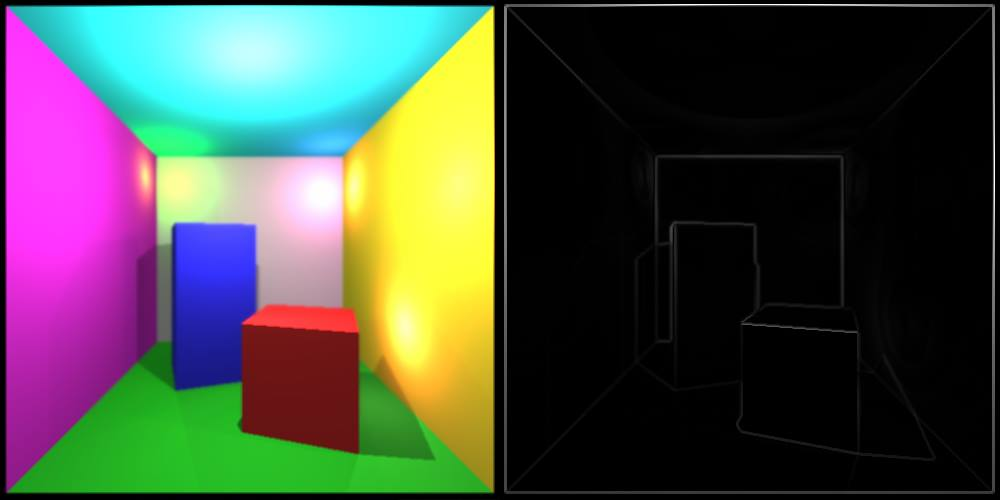
\includegraphics[width=\linewidth]{raytracer_final.jpg}
			\captionsetup{belowskip=4pt,aboveskip=-11pt}
			\caption{Raytracer}
			\label{graph}
		\end{minipage}
	\end{figure}
	
	%----------------------------------------------------------------------------------------
	%	REFERENCES
	%----------------------------------------------------------------------------------------

	\section*{References}
	1. http://www.math.cornell.edu/~andreim/Lec17.pdf
\end{document}